\subsection{Terrain}
\begin{center}
  \textit{User parameters} $\rightarrow$ \textbf{TerrainGenerator}  $\rightarrow$ \textit{Terrain}
\end{center}

We will approach this subproblem by first generating a heightmap that represents the hills and the valleys of the landscape.
A heightmap is a bitmap image where each pixel typically store values representing a surface elevation or displacement.
This is often visualized as a grayscale image where the black pixels represents the minimum height displacement and white the maximum elevation.
To this projects particular use case the pixel values will store the terrain elevation and rendered as a 3D mesh.
One limitation of using a heightmap however, is that it can not represent more complex 3D geometry such as caves or overhangs, but since the main focus of the project is on procedurally generating a city not the terrain this is not deemed as a problem.
Figure~\ref{fig:heightmap} illustrates an example heightmap visualized as a grayscale image.

% NOTE(anton): image generated from https://cpetry.github.io/TextureGenerator-Online/
\begin{figure}[h]
  \centering
  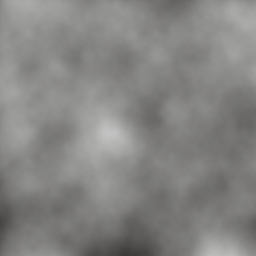
\includegraphics[width=0.25\textwidth]{figure/heightmap.png}
  \caption{An example heightmap generated using Perlin Noise}
  \label{fig:heightmap}
\end{figure}

We plan to generate the heightmap using multiple layers of simplex noise.
Simplex noise is a type of gradient noise commonly used in computer graphics and procedural generation.
The so-called gradient noise is where a psuedo-random gradient(or slope) is generated at regularly spaced points in space.
The points are then interpolated using a smoothing function to achieve a wave-like texture fitting for representing the terrain.
Each octave, or layer, of simplex noise will represent different levels of terrain granularity.
Higher frequency of noise corresponds to an area on the heightmap where we would like to generate an area with a small, yet intense difference in elevation.
Whereas lower frequencies will correspond to areas of a less intense, but larger difference in elevation forming the contour of the terrain.

The color of the terrain will be based on the height levels e.g.\ grasslands near sea level, rocky mountain textures for the taller regions, and snow for top peaks of some of the taller mountains.
One approach for achieving this is a technique called Texture splatting that is commonly used for terrain rendering.
This method consists of combining different textures blended together according to an alphamap, also referred to as a weightmap or splatmap.
Figure~\ref{fig:texture-splatting} demonstrates this technique in action.

\begin{figure}[h]
  \centering
  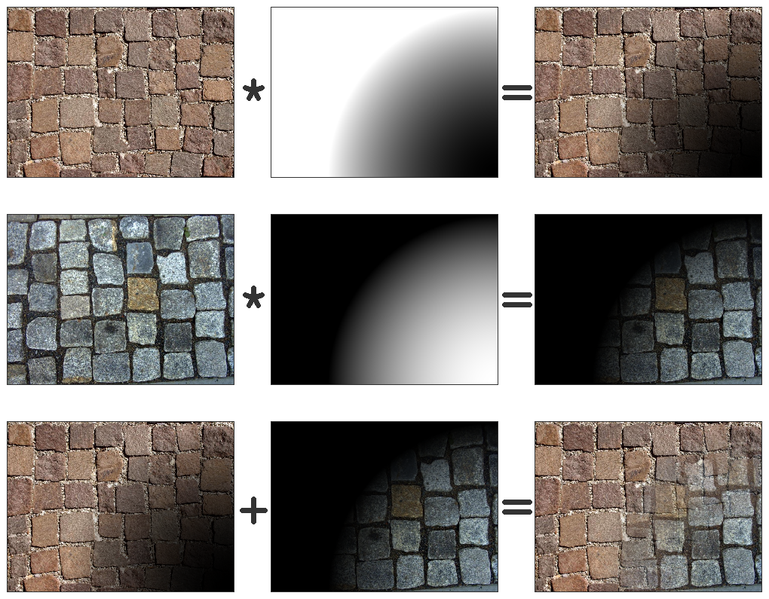
\includegraphics[width=0.4\textwidth]{figure/texture-splatting.png}
  \caption{Example of texture splatting from related work \cite{wiki:texture-splatting-img}}
  \label{fig:texture-splatting}
\end{figure}

Furthermore the user can provide a threshold height for the sea level where any point of the terrain below this threshold value will fill the valley or space with water.

If there is still time after previously mentioned implementations we intend to make the terrain more interesting by generating trees and grass throughout the world.
The way we intend to do this is to use poisson disc sampling to distribute points for trees in a natural looking fashion. % source: https://odr.chalmers.se/handle/20.500.12380/244588

